\documentclass[11pt,a4paper]{article}
%\documentclass{ctexart}

%\usepackage{fontspec, xunicode, xltxtra}
%\setmainfont{Hiragino Sans GB}
\usepackage{xeCJK}
%\setCJKmainfont[BoldFont=STZhongsong, ItalicFont=STKaiti]{STSong}
%\setCJKsansfont[BoldFont=STHeiti]{STXihei}
%\setCJKmonofont{STFangsong}

%使用Xelatex编译

% 设置页面
%==================================================
\linespread{2} %行距
% \usepackage[top=1in,bottom=1in,left=1.25in,right=1.25in]{geometry}
% \headsep=2cm
% \textwidth=16cm \textheight=24.2cm
%==================================================

% 其它需要使用的宏包
%==================================================
\usepackage[colorlinks,linkcolor=blue,anchorcolor=red,citecolor=green,urlcolor=blue]{hyperref} 
\usepackage{tabularx}
\usepackage{authblk}         % 作者信息
\usepackage{algorithm}     % 算法排版
\usepackage{amsmath}     % 数学符号与公式
\usepackage{amsfonts}     % 数学符号与字体
\usepackage{mathrsfs}      % 花体
\usepackage{amssymb}

\usepackage{graphicx} 
\usepackage{graphics}
\usepackage{color}
\usepackage{xcolor}

\usepackage{fancyhdr}       % 设置页眉页脚
\usepackage{fancyvrb}       % 抄录环境
\usepackage{float}              % 管理浮动体
\usepackage{geometry}     % 定制页面格式
\usepackage{hyperref}       % 为PDF文档创建超链接
\usepackage{lineno}          % 生成行号
\usepackage{listings}        % 插入程序源代码
\usepackage{multicol}       % 多栏排版
%\usepackage{natbib}         % 管理文献引用
\usepackage{rotating}       % 旋转文字,图形,表格
\usepackage{subfigure}    % 排版子图形
\usepackage{titlesec}       % 改变章节标题格式
\usepackage{moresize}   % 更多字体大小
\usepackage{anysize}
\usepackage{indentfirst}  % 首段缩进
\usepackage{booktabs}   % 使用\multicolumn
\usepackage{multirow}    % 使用\multirow

\usepackage{wrapfig}
\usepackage{titlesec}     % 改变标题样式
\usepackage{enumitem}
\usepackage{aas_macros}

\newcommand{\myvec}[1]%
   {\stackrel{\raisebox{-2pt}[0pt][0pt]{\small$\rightharpoonup$}}{#1}}  %矢量符号
\renewcommand{\vec}[1]{\boldsymbol{#1}}
\newcommand{\me}{\mathrm{e}}
\newcommand{\mi}{\mathrm{i}}
\newcommand{\dif}{\mathrm{d}}
\newcommand{\tabincell}[2]{\begin{tabular}{@{}#1@{}}#2\end{tabular}}

\def\kpc{{\rm kpc}}
\def\km{{\rm km}}
\def\cm{{\rm cm}}
\def\TeV{{\rm TeV}}
\def\GeV{{\rm GeV}}
\def\MeV{{\rm MeV}}
\def\GV{{\rm GV}}
\def\MV{{\rm MV}}
\def\yr{{\rm yr}}
\def\s{{\rm s}}
\def\ns{{\rm ns}}
\def\GHz{{\rm GHz}}
\def\muGs{{\rm \mu Gs}}
\def\arcsec{{\rm arcsec}}
\def\K{{\rm K}}
\def\microK{\mu{\rm K}}
\def\sr{{\rm sr}}
\newcolumntype{p}{D{,}{\pm}{-1}}

\renewcommand{\figurename}{Fig.}
\renewcommand{\tablename}{Tab.}

\renewcommand{\arraystretch}{1.5}

\setlength{\parindent}{0pt}  %取消每段开头的空格

\title{粒子的运动学描写}
\author{}
\date{\today}
\begin{document}

\maketitle

\section{相对论能动量}
粒子的\textcolor{red}{动量}
\begin{equation}
\vec{p} = \gamma m \vec{u} = \frac{m\vec{u}}{\sqrt{1-\frac{u^2}{c^2}}}
\end{equation}
粒子的\textcolor{red}{能量}
\begin{equation}
E = \gamma m c^2 = \frac{m c^2}{\sqrt{1-\frac{u^2}{c^2}}}
\end{equation}
粒子的\textcolor{red}{静能}
\begin{equation}
E = m c^2
\end{equation}
粒子的\textcolor{red}{动能}
\begin{equation}
T = E - mc^2
\end{equation}
\begin{equation}
E^2 = p^2 c^2 +m^2 c^4
\end{equation}
从任何小于$c$的有限速率增加到或者超过光速是不可能的;若粒子生来就具有大于光速的速率,并不破坏这一说法;

一个自由粒子的能量、动量与速度的关系:
\begin{equation}
\vec{u} = \frac{c^2 \vec{p}}{E}
\end{equation}

\section{能动量四维矢量的洛伦兹变换}
the Lorentz transformation for momentum and energy
\begin{eqnarray}
\nonumber p^{\prime}_x &=& \gamma(p_x -vE/c^2) ~, \\
\nonumber p^{\prime}_y &=& p_y ~, \\
\nonumber p^{\prime}_z &=& p_z ~, \\
E^{\prime} &=& \gamma(E -vp_x)
\end{eqnarray}
the inverse transformation is
\begin{eqnarray}
\nonumber p_x &=& \gamma(p^{\prime}_x +vE^{\prime}/c^2) ~, \\
\nonumber p_y &=& p^{\prime}_y ~, \\
\nonumber p_z &=& p^{\prime}_z ~, \\
E &=& \gamma(E^{\prime} +vp^{\prime}_x)
\end{eqnarray}

洛伦兹不变式
\begin{equation}
E^2 -\vec{p}^2 c^2 = {E^{\prime}}^2 -\vec{p}^2 c^2 = {\rm Const.}
\end{equation}
若系统为单一粒子,其静质量为$m_0$,将$x^{\prime}, y^{\prime}, z^{\prime}$系统固定在$m_0$ 上,即$m_0$粒子在$x^{\prime}, y^{\prime}, z^{\prime}$系内是静止的,其动量$\vec{p}^{\prime} = 0$,则不变式的常量为$m_0^2$
\begin{equation}
E^2 -\vec{p}^2 c^2 = {E^{\prime}}^2 = m_0^2
\end{equation}
对于多粒子系统,其总能量和总动量组成四矢量,在彼此间无相互作用时,洛伦兹不变式为
\begin{eqnarray}
\left(\sum_i E_i  \right)^2 -\left(\sum_i \vec{p}_i  \right)^2 = {\rm Const.}
\end{eqnarray}
在质心系统中,$\sum_i \vec{p}_i^* = 0$,此常量等于$E_{\rm cm}^2 = {E^*}^2 = S$。\textcolor{red}{在一般情况下,此常量并不等于系统的总质量$M_0$}。但若这个多粒子系统是\textcolor{red}{由单一母粒子$M_0$衰变产生的},则这一常量等于\textcolor{red}{母粒子总静止能量的平方$M_0^2$},$M_0$称为这个\textcolor{red}{多粒子系统的不变质量}。




\section{碰撞的相对论运动学}
把质心系适当地推广为洛伦兹参照系,在该参照系内,所有粒子的总的空间线动量对于$0$;这样一个洛伦兹参照系总是能够找到的,因为一个质点系的总四维动量矢量是类时的;

总的四维动量
\begin{equation}
P_{\mu} = \sum_r p_{r\mu}
\end{equation}
\begin{eqnarray}
\nonumber P_{\mu} P_{\mu} = \sum_{r,s} p_{r\mu} p_{s\mu} &=& -\sum_{r} m_r^2 c^2 + \sum_{r \neq s} p_{r\mu} p_{s\mu} ~, \\
&=& -\sum_{r} m_r^2 c^2 + \sum_{r \neq s} m_r m_s \gamma_r \gamma_s (c^2 -\vec{v}_r \cdot \vec{v}_s)
\end{eqnarray}
由于实物粒子的速度始终小于$c$,所以$P_{\mu}$的平方始终是负值;一定会有某种洛伦兹坐标系,它保证被变换矢量$P_{\mu}$的空间分量全部为$0$,这种坐标系称为\textcolor{red}{动量中心系},或者不太严格地称为\textcolor{red}{质心系},“C-O-M”系;

碰撞前后总的四维动量矢量守恒;意味着空间线动量的守恒和总能量(包括静止质能)的守恒;变换到动量中心系和起始于动量中心系的洛伦兹变换;同时构成一些在所有洛伦兹系统内都有相同数值的洛伦兹不变量(世量标量);

考虑由两个粒子引起的反应,它产生出另一组质量为$m_r (r = 3, 4, 5, \cdots)$的粒子,在“C-O-M” 系内,变换后的总动量$P^{\prime}_{\mu}$具有零值空间分量以及一个第四分量$iT^{\prime}/c$。把“C-O-M”系看作是质量为$M=T^{\prime}/c^2$的复合粒子的固有系统或静止系统;$P_{\mu}$量值的平方在所有洛伦兹系统内必定是不变量(并在反应中守恒)。因此
\begin{equation}
P_{\mu} P_{\mu} = P^{\prime}_{\mu}P^{\prime}_{\mu} = -\frac{{E^{\prime}}^2}{c^2} = -M^2 c^2
\end{equation}
对原有粒子,
\begin{equation}
P_{\mu} P_{\mu} = -(m_1^2 +m_2^2) c^2 + 2p_{1\mu} p_{2\mu}
\end{equation}
在“C-O-M”系内的能量或等效质量$M$,可依据入射粒子表达成
\begin{equation}
{E^{\prime}}^2 \equiv M^2 c^4 = (m_1^2 +m_2^2) c^4 +2(E_1 E_2 -c^2 \vec{p}_1 \cdot \vec{p}_2 )
\end{equation}
假设有一个粒子,如粒子2,在实验室系下是静止的,则$\vec{p}_2 = 0$和$T_2 = m_2 c^2$,C-O-M能量为
\begin{equation}
{E^{\prime}}^2 \equiv M^2 c^4 = (m_1^2 +m_2^2) c^4 +2m_2 c^2 E_1 =  (m_1^2 +m_2^2)^2 c^4 +2m_2 c^2 T_1
\end{equation}
C-O-M系内的有效能量仅随入射动能缓慢增加,甚至在运动动能远大于静止质能的“超相对论”区域内,$E^{\prime}$也仅按$T_1$的平方根增加;

在C-O-M系中适用的小数量入射能量按比例增加的效应,是用阈能表示的;有可能引起反应(除了弹性散射)的最低能量是反应物静止在C-O-M系内时的能量。任何有限动能都要求一个较高的$E^{\prime}$,或者说要求一个较高的入射能量;反应后,C-O-M系内的总的四维动量$P_{\mu}^{\prime \prime}$,它在阈值处的量值决定于
\begin{equation}
P_{\mu}^{\prime \prime} P_{\mu}^{\prime \prime} = -c^4 \left(\sum_r m_r \right)^2
\end{equation}
对于静止靶,阈值处入射运动能量决定于
\begin{equation}
\frac{T_1}{m_1 c^2} = \frac{\left(\sum\limits_r m_r \right)^2 -(m_1 +m_2)^2}{2m_1 m_2}
\end{equation}
若反应的$Q$定义为
\begin{equation}
Q  = \sum_r m_r -(m_1 +m_2)
\end{equation}
则
\begin{equation}
\frac{T_1}{m_1 c^2} = \frac{Q^2 +2Q(m_1 +m_2)}{2m_1 m_2}
\end{equation}

实验室系内反应产物在阈值处的能量;C-O-M系是质量$M$的静止系统,它的$P^{\prime}_4 = i M c$,在任何其它系统中,四维矢量的第四分量是$P_4 = i M c \gamma$,但在实验室系内则为
\begin{equation}
P_4 = \frac{i}{c} (E_1 +E_2) = \frac{i}{c} (E_1 +m_2 c^2)
\end{equation}
后一式只对静止靶粒子成立;因此,C-O-M系统相对于实验室系的运动应使
\begin{equation}
\gamma = \frac{E_1 +m_2 c^2}{Mc^2}
\end{equation}
但在阈值处,所有的反应产物在C-O-M系内都是静止的,因此$M = \sum\limits_r m_r$,这时有
\begin{equation}
\gamma = \frac{T_1 +(m_1 +M_2) c^2}{\sum\limits_r m_r c^2}   ~~~~~\text{阈值}
\end{equation}
在实验室系内,第$s$个反应产物的动能是
\begin{equation}
T_s = m_s c^2 (\gamma -1)
\end{equation}

\section{The elastic collision}
\cite{greiner2003classical} Denote the four-momenta of the two particles before the collision by $p$ and $P$, and after the collision by $p^\prime$ and $P^\prime$. The four-momentum conservation law then reads
\begin{equation}
p +P = p^\prime +P^\prime ~,
\end{equation}
The four-vector equation comprises two conservation laws, namely that for the usual three-momentum and that for the energy
\begin{align}
\vec{p} +\vec{P} &= \vec{p}^\prime +\vec{P}^\prime ~, \label{eq:momentum_coserva} \\
e + E &= e^\prime+E^\prime = \overline{E}, \label{eq:energy_coserva}
\end{align}
where with the rest masses of the particles $m_0$ and $M_0$
\begin{align}
e^2 &= m_0^2 c^4 +\vec{p}^2 c^2 ~, \\
E^2 &= M_0^2 c^4 +\vec{P}^2 c^2 ~,
\end{align}
are the energies of the particles before the collision. Because the collision was supposed as elastic, the rest masses $m_0$ and $M_0$ remain unchanged in the collision process. The energies of the particles after the collision are given by $e^\prime$ and $E^\prime$,
\begin{align}
e^{\prime 2} &= m_0^2 c^4 +\vec{p}^{\prime 2} c^2 ~, \\
E^{\prime 2} &= M_0^2 c^4 +\vec{P}^{\prime 2} c^2 ~,
\end{align}
The total energy of the considered system is $\overline{E}$. The rest masses and the components of the initial momenta are to be considered as given. We are looking for the components of the final momenta $\vec{p}^{\prime}$ and $\vec{P}^{\prime}$. Hence, we have four equations for six unknown quantities, such that the general solution will contain two undetermined parameters. 

The collision problem becomes most simple in that coordinate frame where the initial momenta $\vec{p}$ and $\vec{P}$ are oppositely equal. This is the frame in which the total momentum vanishes and therefore the center of mass of the two particles is at rest. This is the rest frame of the center of mass, which is denoted as the \textcolor{red}{\bf center-of-mass system}. The final values $\vec{p}^{\prime}$ and $\vec{P}^{\prime}$ of the momenta must be oppositely equal. The magnitudes $|\vec{p}| = |\vec{P}|$  and $|\vec{p}^{\prime}| = |\vec{P}^{\prime}|$ of the momenta remain unchanged in the collision:
\begin{equation*}
|\vec{p}^{\prime}| = |\vec{p}^{\prime}| ~,
\end{equation*}
or simply
\begin{equation}
p = p^{\prime} ~,
\end{equation}
In the collision process only the straight line along the initial direction of the two momenta is arbitrarily rotated in space (see Figure (\ref{fig:elastic_collision})). 

%===========================================================================================================================
\begin{figure*}
\centering
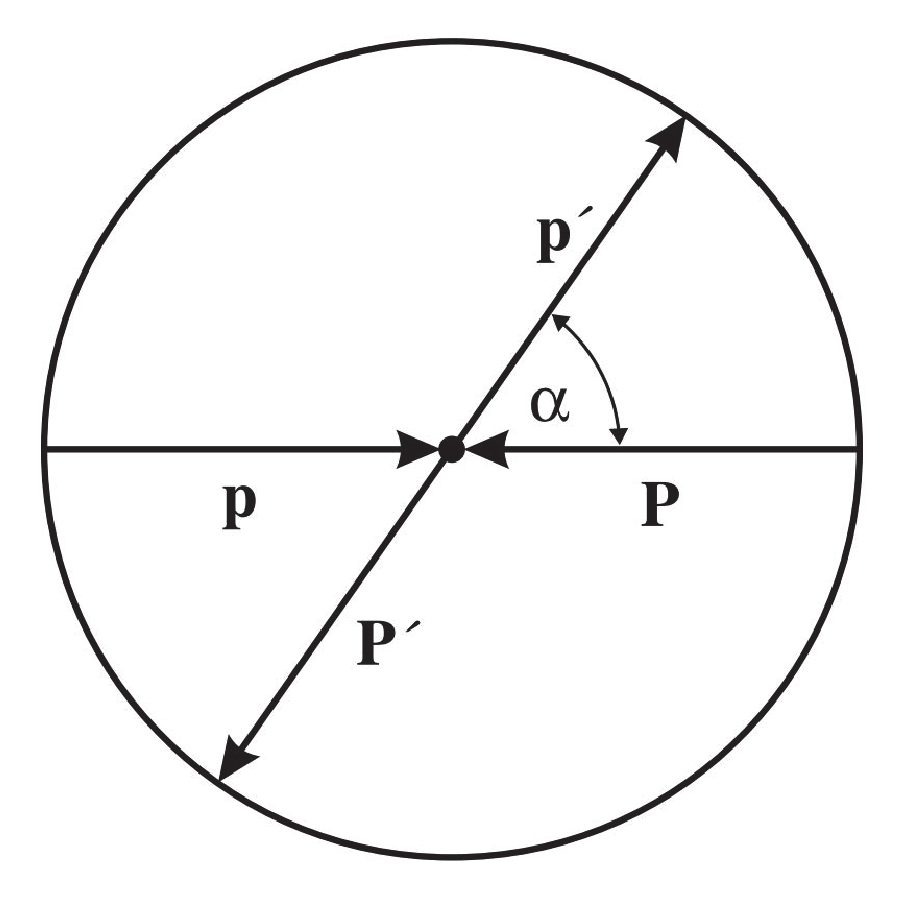
\includegraphics[height=5.cm, angle=0]{elastic_collision.eps}
\caption{
The elastic collision in the center-of-mass system. 
}
\label{fig:elastic_collision}
\end{figure*}
%===========================================================================================================================

The deflection angle $\alpha$ represents one of the undefined parameters. The second parameter is the azimuth angle specifying the position of the plane defined by $\vec{p}$ and $\vec{p}^\prime$, which evidently may be arbitrarily rotated about the direction of $\vec{p}$.  One of the particles is at rest before the collision:
\begin{equation}
\vec{P} = 0 ~.
\end{equation}
Eq. (\ref{eq:momentum_coserva}) simplifies to 
\begin{equation}
\vec{p} = \vec{p}^\prime +\vec{P}^\prime ~.
\end{equation}
The energy equation is
\begin{equation}
\dfrac{E}{c} = M_0 c ~.
\end{equation}
One may choose the angle $\theta$ or $\alpha$ as the first undetermined parameter (Figure (\ref{fig:Momentum_balance})). The second parameter is again the azimuth angle, which determines the position of the drawing plane of the figure that may be arbitrarily rotated about the direction of $\vec{p}$.
\begin{align}
& P^{\prime 2} = p^{\prime 2} +p^2 -2 p p^\prime \cos \theta ~, \\
& \varepsilon - \sqrt{M_0^2 c^2 +P^{\prime 2} } = \sqrt{m_0^2 c^2 +p^{\prime 2} } ~,
\end{align}
where $\varepsilon = \overline{E}/c$.

%===========================================================================================================================
\begin{figure*}
\centering
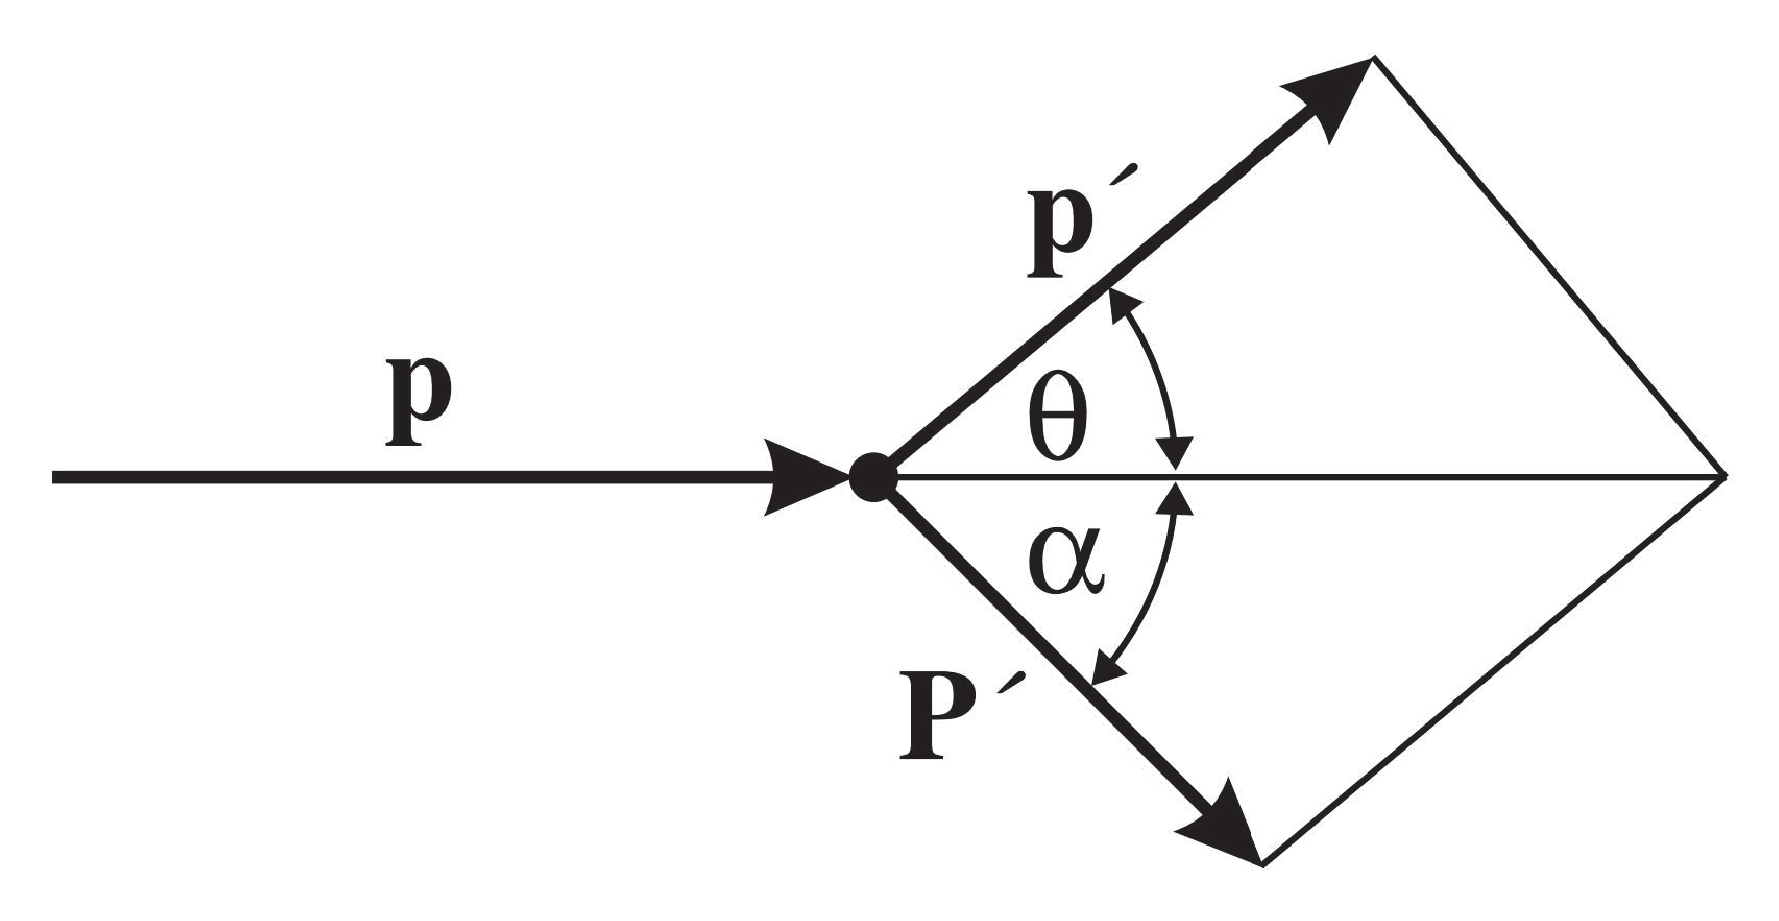
\includegraphics[height=5.cm, angle=0]{Momentum_balance.eps}
\caption{
Momentum balance of a colliding particle and a particle at rest.
}
\label{fig:Momentum_balance}
\end{figure*}
%===========================================================================================================================

\begin{equation*}
p^{\prime 2} +m_0^2 c^2 = P^{\prime 2} +M_0^2 c^2 +\varepsilon^2 -2\varepsilon \sqrt{M_0^2 c^2 +P^{\prime 2} } ~.
\end{equation*}
\begin{align*}
& (m_0^2 c^2-M_0^2 c^2-p^2 -\varepsilon^2 +2 p p^\prime \cos \theta)^2 - 4\varepsilon^2 (M_0^2 c^2 +p^2 +p^{\prime 2} - 2p p^\prime \cos \theta) = 0 ~, \\
& 4(p^2 \cos \theta-\varepsilon^2) p^{\prime 2} +4 p p^\prime \cos\theta (m_0^2 c^2 -M_0^2 c^2 -p^2 +\varepsilon^2) \\
& +(m_0^2 c^2 -M_0^2 c^2)^2 -2(p^2 +\varepsilon^2)m_0^2 c^2 +(\varepsilon^2 -p^2) M_0^2 c^2 +(p^2 -\varepsilon^2)^2 = 0 ~.
\end{align*}
By making use of the relations
\begin{align}
\varepsilon &= \sqrt{p^2 +m_0^2 c^2} +M_0 c ~, \\
\varepsilon &= \dfrac{e}{c} +M_0 c ~.
\end{align}
\begin{align}
\nonumber & \left(\left(\dfrac{e}{c} +M_0c \right)^2 -p^2 \cos \theta \right) p^{\prime 2} -2 p p^\prime \cos \theta \left(m_0^2 c^2 +M_0 c\sqrt{p^2 +m_0^2 c^2} \right) -p^2 c^2 (M_0^2 -m_0^2) = 0 ~. \\
\nonumber & \left(\left(\dfrac{e}{c} +M_0c \right)^2 -p^2 \cos \theta \right) p^{\prime 2} -2 p p^\prime \cos \theta \left(m_0^2 c^2 +M_0 c\dfrac{e}{c} \right) -p^2 c^2 (M_0^2 -m_0^2) = 0 ~. \\
& p^\prime = \dfrac{p}{(M_0c +e/c)^2 -p^2 \cos^2 \theta} \left\{\cos \theta \left(m_0^2 c^2  +M_0 c \dfrac{e}{c} \right) \pm \left(\dfrac{e}{c} c +M_0 c^2 \right) \sqrt{M_0^2 -m_0^2 \sin^2 \theta}   \right\} ~.
\end{align}
For $M_0 > m_0$ only the positive sign before the square root must be admitted. $\varepsilon > p$ and therefore $\varepsilon^2 -p^2 \cos^2 \theta > 0$. In the case $M_0 < m_0$, the angle $\theta$ passes twice through the range $0 \leqslant \theta \leqslant \theta_{\rm max}$, whereby $\theta_{\rm max}$ follows from
\begin{equation*}
M_0 = m_0 \sin \theta_{\rm max} ~.
\end{equation*}
To any angle $\theta$ in this range will correspond two solutions of the collision problem. In the case $M_0 > m_0$, however, $\theta$ passes the range $0 \leqslant \theta \leqslant \pi$ once, hence for any value of $\theta$ there is only one solution.
\begin{equation}
\dfrac{e^\prime}{c} = \dfrac{1}{(M_0c+e/c)^2 -p^2 \cos^2 \theta} \left\{\left(\dfrac{e}{c} +M_0 c \right) \left(M_0 c\dfrac{e}{c} +m_0^2 c^2 \right) \pm cp^2 \cos \theta \sqrt{M_0^2 -m_0^2 \sin^2 \theta}  \right\}
\end{equation}
\begin{equation}
\dfrac{E^\prime}{c} = M_0 c +\dfrac{e}{c}  -\dfrac{e^\prime}{c} ~.
\end{equation}

\section{Kinematic Variables}

\subsection{Light-Cone Variables}
\cite{cheuk1994introduction} In many high-energy reaction processes, a detected particle can be identified as originating from one of the colliding particles. For example, in the reaction
\begin{equation}
b+a \rightarrow c +X ~,
\end{equation}
where $c$ is a detected particle, $c$ may sometimes be considered as fragmenting from the incident beam particle $b$ or from the target particle $a$.

A reaction in which the detected particle $c$ is described as originating from the beam particle $b$ is called a projectile fragmentation reaction. The region of the momentum of $c$ in which this type of reaction is dominant is referred to as the projectile fragmentation region. It lies in the forward direction with respect to the beam axis. Similarly, a reaction in which the detected particle $c$ can be described as originating from the target particle a is called a target fragmentation reaction. The kinematic region in which this type of reaction is dominant is the target fragmentation region, which is near the region of momentum where the target particle is initially at rest. 

In a reaction, kinematic quantities along the direction of the incident beam, which we shall identify as the longitudinal axis, have properties quite different from those along the transverse directions perpendicular to the beam axis. We shall designate the longitudinal axis as the z-axis. For convenience, we use the same symbol to represent a particle and its four-momentum. For example, $c = (c_0, \vec{c}_T, \vec{c}_z)$, where $c_0$ is the energy of the particle $c$, $c_z$ is its longitudinal momentum and $c_T$ is its two-dimensional transverse momentum in the plane perpendicular to the longitudinal axis. 

Two linear combinations of $c_0$ and $c_z$ have special properties under a Lorentz transformation in the $z$-direction. The quantity
\begin{equation}
c_+ = c_0 +c_z ~,
\end{equation}
is called the forward light-cone momentum of $c$, while the quantity
\begin{equation}
c_- = c_0 -c_z ~,
\end{equation}
is called the backward light-cone momentum of $c$. For an energetic particle traveling in the forward direction (along the beam direction), its forward light-cone momentum $c_+$ is large, while its backward light-cone momentum $c_-$ is small. Conversely, for a particle traveling in the backward direction opposite to that of the beam, its backward light-cone momentum is large, while its forward light-cone momentum is small.






\section{习题}
1. 在实验室系中,静质量为$m_1$、动量为$\vec{p}_1$、能量为$E_1$的粒子撞击静质量为$m_2$ 的静止粒子;在质心系中,$m_1$的动量为$\vec{p}^{\prime}_1$,这两个粒子的总能量为$E^{\prime}$。 试证明:\\
1). ${E^{\prime}}^2 = m_1^2 c^4 + m_2^2 c^4 +2m_2 c^2 E_1$;\\
2). $\vec{p}^{\prime}_1 = \frac{m_2 c^2}{E^{\prime}} \vec{p}_1$;\\
3). 描述质心C在实验室系中速度$v_c$的洛伦兹变换参量为
\begin{equation*}
\beta_c = \frac{\vec{v}_c}{c} = \frac{\vec{p}_1c }{m_2 c^2 +E_1}, \gamma_c = \frac{m_2 c^2 +E_1}{E^{\prime}}
\end{equation*}
4). 当趋于非相对论极限时,上面的结果分别化为熟知的公式:
\begin{equation*}
E^{\prime} = m_1 c^2 +m_2 c^2 +\frac{m_2}{m_1 +m_2} \frac{p_1^2}{2m_1} ~,~ \vec{p}^{\prime}_1 = \frac{m_2}{m_1 +m_2} \vec{p}_1 ~,~ \vec{\beta}_c = \frac{\vec{v}_c}{c} = \frac{\vec{p}_1}{(m_1 +m_2) c}
\end{equation*}

证:1). 实验室系,系统的四维动量为
\begin{equation*}
P = \left[\vec{p}_1 +\vec{p}_2, \frac{i}{c} (E_1 +E_2) \right] = \left[\vec{p}_1, \frac{i}{c} (E_1 +m_2 c^2) \right]
\end{equation*}
质心系,系统的四维动量为
\begin{equation*}
P^{\prime} = \left[\vec{p}^{\prime}_1 +\vec{p}^{\prime}_2, \frac{i}{c} (E^{\prime}_1 +E^{\prime}_2) \right] = \left[ 0, \frac{i}{c} E^{\prime} \right]
\end{equation*}
\begin{equation*}
P^{\prime}_{\mu} P^{\prime}_{\mu} = -\frac{{E^{\prime}}^2}{c^2} = P_{\mu} P_{\mu} = p_1^2 - \left(\frac{E_1 +m_2 c^2}{c} \right)^2
\end{equation*}
得到
\begin{equation*}
{E^{\prime}}^2 = m_1^2 c^4 + m_2^2 c^4 +2m_2 c^2 E_1
\end{equation*}

2). 在质心系下,
\begin{equation*}
E^{\prime} = E^{\prime}_1 +E^{\prime}_2 = \sqrt{{p^{\prime}}^2_1 c^2 +m_1^2 c^4} +\sqrt{{p^{\prime}}^2_2 c^2 +m_2^2 c^4}
\end{equation*}
\begin{equation*}
(E^{\prime} -\sqrt{{p^{\prime}}^2_1 c^2 +m_1^2 c^4})^2  = {p^{\prime}}^2_2 c^2 +m_2^2 c^4
\end{equation*}
\begin{equation*}
{E^{\prime}}^2 + {p^{\prime}}^2_1 c^2 +m_1^2 c^4 - 2 E^{\prime} \sqrt{{p^{\prime}}^2_1 c^2 +m_1^2 c^4} = {p^{\prime}}^2_2 c^2 +m_2^2 c^4
\end{equation*}
由1).得到的关系
\begin{equation*}
{E^{\prime}}^2 = m_1^2 c^4 + m_2^2 c^4 +2m_2 c^2 E_1 = E_{10}^2 +E_{20}^2 +2E_1 E_{20}
\end{equation*}
带入上式,得到
\begin{equation*}
\left(\frac{m_1^2 c^4 + m_2 c^2 E_1}{E^{\prime}} \right)^2 = {p^{\prime}}^2 c^2 +m_1^2 c^4
\end{equation*}
\begin{equation*}
\frac{E_{10}^4 +E_{20}^2 E_1^2 +2E_{10}^2 E_{20} E_1}{{E^{\prime}}^2} = {p^{\prime}}^2 c^2 +E_{10}^2
\end{equation*}
\begin{equation*}
{p^{\prime}}^2c^2 = \frac{E_{20}^2 (E_1^2 -E_{10}^2)}{{E^{\prime}}^2}
\end{equation*}
\begin{equation*}
p^{\prime} = \frac{m_2 c^2}{E^{\prime}} p_1
\end{equation*}
由于$\vec{p}^{\prime}_1$与$\vec{p}_1$同方向,故
\begin{equation*}
\vec{p}^{\prime} = \frac{m_2 c^2}{E^{\prime}} \vec{p}_1
\end{equation*}

3). 质心C在实验室系中的速度为$\vec{v}_c$,则
\begin{equation*}
\vec{p}^{\prime}_1 = -\vec{p}^{\prime}_2 = \frac{m_2 \vec{v}_c}{\sqrt{1- v_c^2/c^2}}
\end{equation*}
而由2).
\begin{equation*}
\vec{p}^{\prime} = \frac{m_2 c^2}{E^{\prime}} \vec{p}_1
\end{equation*}
令
\begin{equation*}
\vec{\beta}_c = \frac{\vec{v}_c}{c}
\end{equation*}
可以得到
\begin{equation*}
\frac{\beta_c^2}{1-\beta_c^2} = \frac{p^2_1 c^2}{{E^{\prime}}^2}
\end{equation*}
\begin{equation*}
\frac{{E^{\prime}}^2 +p_1^2 c^2}{{E^{\prime}}^2} \beta_c^2 = \frac{p_1^2 c^2}{{E^{\prime}}^2}
\end{equation*}
化简得
\begin{equation*}
\beta_c^2 = \frac{p_1^2 c^2}{{E^{\prime}}^2 +p_1^2 c^2} = \frac{p_1^2 c^2}{(m_2 c^2 +E_1)^2}
\end{equation*}
由于$\vec{p}_1$与$\vec{v}_c$同方向,故
\begin{equation*}
\vec{\beta}_c =  \frac{\vec{p}_1 c}{m_2 c^2 +E_1}
\end{equation*}
同时
\begin{equation*}
\gamma_c = \frac{1}{\sqrt{1 -\beta^2_c}} = \frac{m_2 c^2 +E_1}{E^{\prime}}
\end{equation*}

4). 非相对论极限下,$pc \ll mc^2$,
\begin{eqnarray*}
\nonumber {E^{\prime}}^2 &=& m_1^2 c^4 + m_2^2 c^4 +2m_2 c^2 E_1 ~, \\
&=& m_1^2 c^4 + m_2^2 c^4 +2m_2 c^2 (m_1 c^2 +\frac{p_1^2}{2m_1}) ~, \\
&=& (m_1+ m_2)^2 c^4 +\frac{m_2}{m_1}  p_1^2 c^2 ~,
\end{eqnarray*}
\begin{eqnarray*}
\nonumber E^{\prime} &=& (m_1+ m_2) c^2 \left(1 + \frac{m_2}{m_1}  \frac{p_1^2 c^2}{(m_1+ m_2)^2 c^4}\right)^{1/2} ~, \\
\nonumber &\sim& (m_1+ m_2) c^2 + \frac{m_2}{m_1+ m_2} \frac{p_1^2}{2m_1}
\end{eqnarray*}


\begin{eqnarray*}
\nonumber \vec{p}^{\prime} &=& \frac{m_2 c^2}{E^{\prime}} \vec{p}_1 ~, \\
\nonumber &=& \frac{m_2 c^2}{\sqrt{m_1^2 c^4 + m_2^2 c^4 +2m_2 c^2 E_1}} \vec{p}_1 ~, \\
\nonumber  &\sim& \frac{m_2 c^2}{\sqrt{m_1^2 c^4 + m_2^2 c^4 +2m_2 c^2 m_1 c^2}} \vec{p}_1 ~, \\
&=& \frac{m_2}{m_1 + m_2} \vec{p}_1 ~,
\end{eqnarray*}

\begin{eqnarray*}
\nonumber \vec{\beta}_c &=&  \frac{\vec{p}_1 c}{m_2 c^2 +E_1} ~, \\
\nonumber &\sim& \frac{\vec{p}_1 c}{m_2 c^2 +m_1 c^2} ~, \\
\nonumber &=&  \frac{\vec{p}_1}{(m_1 +m_2) c} ~,
\end{eqnarray*}

2. 在一个碰撞过程中,在实验室中静止质量为$m_2$的一个粒子,被质量为$m_1$、动量为$\vec{p}_1$、 总能量为$E_1$的一个粒子所撞击。在碰撞中,这两个初始粒子转变成质量为$m_3$ 和$m_4$的另外两个粒子。\\
a). 利用不变标积,试证:在动量中心参照系中,总能量$W$的平方由下式给出
\begin{equation*}
W^2 = m_1^2 c^4 +m_2^2 c^4+2m_2 c^2 E_1
\end{equation*}
动量中心参照系中三元动量$\vec{p}^{\prime}_1$是
\begin{equation*}
\vec{p}^{\prime}_1 = \frac{m_2 c^2}{W} \vec{p}_1
\end{equation*}
b). 试证:描述动量中心参照系在实验室系中的速度的洛伦兹变换参量为
\begin{equation*}
\beta_c = \frac{\vec{v}_c}{c} = \frac{\vec{p}_1c }{m_2 c^2 +E_1}, \gamma_c = \frac{m_2 c^2 +E_1}{W}
\end{equation*}
c). 试证:在非相对论极限下,上面的结果分别化为熟知的公式:
\begin{eqnarray*}
W &\simeq& m_1 c^2 +m_2 c^2 +\frac{m_2}{m_1 +m_2} \frac{p_1^2}{2m_1} ~, \\
\vec{p}^{\prime}_1 &\simeq& \frac{m_2}{m_1 +m_2} \vec{p}_1 ~, \\
\vec{\beta}_c &\simeq& \frac{\vec{p}_1}{(m_1 +m_2) c}
\end{eqnarray*}


3. 在一个弹性散射过程中,入射粒子将能量传给静靶。入射粒子失去的能量$\Delta E$作为靶的反冲动能出现,按上题的记号,$m_3 = m_1$和$m_4 = m_2$,而$\Delta E = T_4 = E_4 -m_4$。\\
a). 试证:$\Delta E$可以用下列不同的方法表示,
\begin{eqnarray*}
\Delta E &=& \frac{m_2 c^2}{W^2} p^2_1 (1 -\cos \theta^{\prime}) ~, \\
\Delta E &=& \frac{2m_2 p^2_1 \cos^2 \theta_4}{W^2 +p^2_1 \sin^2 \theta_4} ~, \\
\Delta E &=& \frac{Q^2}{2m_2} ~,
\end{eqnarray*}
这里$Q^2 = -(p_1 -p_3)^2 = (\vec{p}_1 -\vec{p}_3)^2 -(E_1 -E_3)^2$是洛伦兹不变的动量转移(平方);\\
b). 试证:当带电粒子(电子除外)入射到静止电子上时($m_1 \gg m_2$),最大能量损失约为
\begin{equation*}
\Delta E_{\rm max} \simeq 2\gamma^2 \beta^2 m_e
\end{equation*}
式中$\gamma$和$\beta$分别表示入射粒子特性的量,且$\gamma \ll (m_1/m_2)$。考虑入射粒子的静止参照系中有关的碰撞,然后又变回到实验室参照系,从而给上一结果以简单的解释;\\
c). 试证:电子—电子碰撞时的最大能量转移为
\begin{equation*}
\Delta E_{\rm max}^{(e)} = (\gamma -1) m_e
\end{equation*}

证:a). 设出射后的粒子$m_1$,在实验室系中的能量为$E^{\prime \prime}_1$,它与动量中心系$[E^{\prime}_1, \vec{p}^{\prime}_1]$的关系是
\begin{equation*}
E^{\prime \prime}_1 = \gamma_c (E^{\prime}_1 +v_c p^{\prime}_{1x}) = \gamma_c (E^{\prime}_1 +v_c p^{\prime}_{1} \cos \theta^{\prime})
\end{equation*}
其中
\begin{eqnarray*}
\vec{\beta}_c &=&  \frac{\vec{p}_1 c}{m_2 c^2 +E_1} ~, \\
\gamma_c &=& \frac{m_2 c^2 +E_1}{E^{\prime}} ~,
\end{eqnarray*}
代入后得到
\begin{eqnarray*}
E^{\prime \prime}_1 = \frac{E_{20} +E_1}{E^{\prime}} \left(E^{\prime}_1 +p^{\prime}_{1} c \cdot \frac{p_1 c}{E_{20} +E_1} \cos \theta^{\prime}  \right)
\end{eqnarray*}
由于
\begin{equation*}
p^{\prime}_{1} = \frac{E_{20} p_1}{E^{\prime}} ~,
\end{equation*}
\begin{eqnarray*}
E^{\prime \prime}_1 = \frac{E_{20} +E_1}{E^{\prime}} \left(E^{\prime}_1 +\frac{E_{20} p^2_1 c^2}{E^{\prime}(E_{20} +E_1)} \cos \theta^{\prime}  \right)
\end{eqnarray*}
也就是
\begin{eqnarray*}
\frac{E_{20} +E_1}{E^{\prime}} E^{\prime}_1 - E^{\prime \prime}_1 = - \frac{E_{20}}{{E^{\prime}}^2}   p^2_1 c^2 \cos \theta^{\prime}
\end{eqnarray*}
洛伦兹不变量在动量中心系中
\begin{eqnarray*}
E^{\prime} = E^{\prime}_1 +E^{\prime}_2
\end{eqnarray*}
平方后得到
\begin{eqnarray*}
{E^{\prime}}^2 + {E^{\prime}}^2_1 -2E^{\prime} E^{\prime}_1 &=& {E^{\prime}}^2_2 ~, \\
2E^{\prime} E^{\prime}_1 &=& {E^{\prime}}^2 +E_{10}^2 -E_{20}^2 ~, \\
E^{\prime}_1 &=& \frac{{E^{\prime}}^2 +E_{10}^2 -E_{20}^2}{2E^{\prime}} ~, \\
&=& \frac{E_{10}^2 +E_{20} E_1}{E^{\prime}} ~,
\end{eqnarray*}
代入后得到
\begin{eqnarray*}
\frac{E_{20} +E_1}{E^{\prime}} \frac{E_{10}^2 +E_{20} E_1}{E^{\prime}} -E^{\prime \prime}_1 &=& - \frac{E_{20}}{{E^{\prime}}^2}   p^2_1 c^2 \cos \theta^{\prime} ~, \\
\frac{E_{20} p^2_1 c^2 +(E_{20} +E_1)(E_{10}^2 +E_{20} E_1)}{{E^{\prime}}^2}  -E^{\prime \prime}_1 &=& \frac{E_{20}}{{E^{\prime}}^2}  p^2_1 c^2 (1 -\cos \theta^{\prime}) ~, \\
E_1 - E^{\prime \prime}_1 &=&  \frac{E_{20}}{{E^{\prime}}^2}  p^2_1 c^2 (1 -\cos \theta^{\prime})
\end{eqnarray*}
即
\begin{eqnarray*}
\Delta E =  \frac{E_{20}}{{E^{\prime}}^2}  p^2_1 c^2 (1 -\cos \theta^{\prime})
\end{eqnarray*}

4. 一原子核基态静质量为$M$,激发态比基态能量高$\Delta E$,已知$\Delta E \ll Mc^2$,以致$\left(\dfrac{\Delta E}{Mc^2}\right)^2$项可以略去。1.) 试求下列两种情况下光子的频率。i)该核处于基态且静止时吸收一个光子;ii)该核处于激发态且静止时发射一个光子;2.) 论证:处在激发态的静止核所辐射出的光子,不能被处在基态的同类静止核吸收。

解:i)
\begin{eqnarray*}
\vec{p}_1 &=& \dfrac{h \nu_1}{c} \vec{\hat{k}}~\\
\sqrt{(p_1c)^2 +(Mc^2 +\Delta E)^2} &=& h\nu_1 +Mc^2
\end{eqnarray*}
得到
\begin{equation*}
2Mc^2 h\nu_1 = \Delta E (2Mc^2 +\Delta E)
\end{equation*}
光子的频率为
\begin{equation*}
\nu_1 = \frac{\Delta E}{h}\left(1+\frac{\Delta E}{2Mc^2} \right)
\end{equation*}

ii)
\begin{eqnarray*}
\vec{p}_1 + \dfrac{h \nu_1}{c} \vec{\hat{k}} = 0~\\
Mc^2 +\Delta E = \sqrt{(p_1c)^2 +M^2c^4} + h\nu_1
\end{eqnarray*}
得到
\begin{equation*}
2(Mc^2 + \Delta E)h\nu_1 = \Delta E (2Mc^2 +\Delta E)
\end{equation*}
光子的频率为
\begin{eqnarray*}
\nu_1 &=& \dfrac{\Delta E}{2h} \dfrac{2Mc^2 +\Delta E}{Mc^2 + \Delta E} = \dfrac{\Delta E}{h} \left(1+\dfrac{\Delta E}{2Mc^2} \right) \left(1- \dfrac{\Delta E}{Mc^2}\right) ~,\\
&=& \dfrac{\Delta E}{h} \left(1-\dfrac{\Delta E}{2Mc^2} \right)
\end{eqnarray*}

2)处于激发态的静止核发出的光子能量为$\dfrac{\Delta E}{h} \left(1-\dfrac{\Delta E}{2Mc^2} \right)$,而处在基态的同类静止核所吸收的光子能量为$\dfrac{\Delta E}{h} \left(1+\dfrac{\Delta E}{2Mc^2} \right)$,故不能被吸收。

5. 有两个完全相同的物体$A$和$B$,每个的静质量都是$m_0$,$B$静止不动,$A$以速度$u$与$B$发生对心碰撞,碰后粘成一个物体$C$,试求$C$的静质量。

解:
\begin{eqnarray*}
\dfrac{m_0 u}{\sqrt{1-\dfrac{u^2}{c^2}}}  &=& \dfrac{M_0U}{\sqrt{1-\dfrac{U^2}{c^2}}} \\
\dfrac{m_0 c^2}{\sqrt{1-\dfrac{u^2}{c^2}}}  + m_0 c^2 &=& \dfrac{M_0 c^2}{\sqrt{1-\dfrac{U^2}{c^2}}}
\end{eqnarray*}

\begin{equation*}
U = \frac{u}{1+\sqrt{1-\dfrac{u^2}{c^2} } }
\end{equation*}

\begin{eqnarray*}
M_0 &=& m_0 \left(1+\frac{1}{\sqrt{1-\dfrac{u^2}{c^2}} }  \right) \sqrt{1-\frac{U^2}{c^2}} ~,\\
&=& \sqrt{2} m_0  \sqrt{\left(1+\frac{1}{\sqrt{1-\dfrac{u^2}{c^2}} }  \right)}
\end{eqnarray*}

6. 有两个完全相同的物体$A$和$B$,每个的静质量都是$m_0$,在它们发生对心碰撞后,粘合处一个物体$C$,在质心系观测,碰前$A$和$B$的速度大小都是$u$,试求$C$的静质量:1.) 用质心系求解;2.) 用相对于$B$静止的参考系求解。

解:1.) 质心系,动量守恒,碰后产生的$C$静止,由能量守恒
\begin{equation*}
M_0 c^2 = \frac{2m_0 c^2}{\sqrt{1-\dfrac{u^2}{c^2}} }
\end{equation*}

\begin{equation*}
M_0 = \frac{2m_0}{\sqrt{1-\dfrac{u^2}{c^2}} }
\end{equation*}

2.) 以质心系为$\Sigma$系,相对于$B$静止的参考系为$\Sigma^{\prime}$系,则在$\Sigma^{\prime}$ 系中,$A$的速度为
\begin{equation*}
u_A^{\prime} = \frac{2u}{1+\dfrac{u^2}{c^2}}
\end{equation*}

$C$的速度为
\begin{equation*}
U^{\prime} = u
\end{equation*}
在$\Sigma^{\prime}$系中,动量守恒和能量守恒
\begin{eqnarray*}
\frac{m_0 u_A^{\prime } }{\sqrt{1-\dfrac{u_A^{\prime 2}}{c^2}} } &=& \frac{M_0 U^{\prime}}{\sqrt{1-\dfrac{U^2}{c^2}} }\\
\frac{m_0 c^2}{\sqrt{1-\dfrac{u_A^{\prime 2}}{c^2}} } +m_0 c^2 &=& \frac{M_0 c^2}{\sqrt{1-\dfrac{U^2}{c^2}} }
\end{eqnarray*}


\begin{eqnarray*}
M_0 &=& m_0 \left(1 + \frac{1+\dfrac{u^2}{c^2}}{1-\dfrac{u^2}{c^2}}  \right) \sqrt{1 -\dfrac{u^2}{c^2}} \\
&=& \frac{2 m_0 }{\sqrt{1-\dfrac{u^2}{c^2}}}
\end{eqnarray*}













%%%%%%%%%%%%%%%%%%%%%%%%%%%%%%%%%%%%%%%%%%%%%%%%%%%%%%%%%%%%%%%%%%%%%%
\bibliographystyle{unsrt_update}
\bibliography{ref}
%%%%%%%%%%%%%%%%%%%%%%%%%%%%%%%%%%%%%%%%%%%%%%%%%%%%%%%%%%%%%%%%%%%%%%


\end{document}
